\newsubfloat{figure}

\section*{Abstract} % abstract
\paragraph{Background}
Over the last ten years, there has been explosive development in methods
for measuring gene expression. These methods can identify thousands of
genes altered between conditions, but understanding these datasets and forming
hypotheses based on them remains challenging. One way to analyze these datasets
is to associate ontologies (hierarchical, descriptive vocabularies
with controlled relations between terms) with genes and to look for enrichment
of specific terms. Although Gene Ontology (GO) is available for
\emph{Caenorhabditis~elegans}, it does not include anatomical information.
\paragraph{Results}
We have developed a tool for identifying  enrichment of \emph{C.~elegans} tissues
among gene sets and generated a website GUI where users can access this tool.
Since a common drawback to ontology enrichment analyses is its verbosity, we
developed a very simple filtering algorithm to reduce the ontology size by an
order of magnitude. We adjusted these filters and validated our tool using a set
of 30  gold standards from Expression Cluster data in WormBase. We show our tool
can even discriminate between embryonic and larval tissues and can even identify
tissues down to the single-cell level. We used our tool to identify multiple
neuronal tissues that are down-regulated due to pathogen infection in
\emph{C.~elegans}.
\paragraph{Conclusions}
Our Tissue Enrichment Analysis (TEA) can be found within WormBase, and can be
downloaded using Python's standard pip installer. It tests a slimmed-down
\emph{C.~elegans} tissue ontology for enrichment of specific terms and provides
users with a  text and graphic representation of the results.

\section*{Background}
	RNA-seq and other high-throughput methods in biology have the ability to
  identify thousands of genes that are altered between conditions. These genes
  are often correlated in their biological characteristics or functions, but
  identifying these functions remains challenging. To interpret these long lists
  of genes, biologists need to abstract genes into concepts that are biologically
  relevant to form hypotheses about what is happening in the system. One such
  abstraction method relies on Gene Ontology (GO). GO provides a controlled set
  of hierarchically ordered terms~\citep{TheGeneOntologyConsortium2000a,
  TheGeneOntologyConsortium2015} that provide detailed descriptions about the
  molecular, cellular or biochemical functions of any gene. For a given gene
  list, existing software programs can query whether a particular term is
  enriched~\citep{Mi2009, McLean2010, Huang2009, Pathan2015}. One area of
  biological significance that GO does not include is anatomy. One way to
  address this shortcoming is to use a `tissue ontology' that provides a
  complete anatomical description for an organism (e.g.`tissue', `organ' or
  `specific cell'), in this case for \emph{C.~elegans}. Such an ontology has
  been described previously for this organism~\citep{Lee2003}. Cells and tissues
  are physiologically relevant units with broad, relatively well-understood
  functionalities amenable to hypothesis formation. The \emph{C.~elegans}
  database, WormBase~\citep{Howe2016}, maintains a curated list of gene expression
  data from the literature. Here we provide a new framework that analyzes a
  user-input list for enrichment of specific cells and tissues.

Another problem frequently associated with GO enrichment analysis is that it
is often difficult to interpret due to the large number of terms associated with
a given gene (which we refer to as `result verbosity'). DAVID, a common tool for
GO enrichment analysis, clusters enriched terms into broad
categories~\citep{Huang2007}, whereas PANTHER~\citep{Mi2009, Mi2013} attempts to
solve this issue by employing a manually reduced ontology, GOslim (pers.\_ comm.,
H. Yu and P. Thomas). To reduce verbosity, we have filtered our ontology using
a small set of well-defined criteria to remove terms that do not contribute
additional information. To our knowledge, such filtering has not been performed
in an algorithmic fashion for a biological ontology before; indeed, DAVID does
not employ term trimming \emph{a priori} of testing, but rather fuzzy clustering
\emph{post} testing to reduce the number of ontology terms. Other pruning methods
do exist (see for example~\citep{Kim2007, Garrido2012}), but the pruning is
query-dependent or generates a brand new `brief ontology' which satisfies a set
of logic relationships and has certain connectivity requirements. We do not
propose to regenerate a new `brief ontology', but instead we use our approach
to select those nodes that have sufficient annotated evidence for statistical
testing. We believe our trimming methodology strikes a good balance between
detailed tissue calling and conservative testing.

We have developed a tool that tests a user-provided list of genes for term
enrichment using a nematode-specific tissue ontology. This ontology, which is
not a module of Gene Ontology, is verbose. We select nodes from the ontology for
statistical testing using an algorithmic approach, outlined below, that reduces
multiple hypothesis testing issues by limiting testing to terms that are
well-annotated. The results are provided to the user in a GUI that includes a
table of results and an automatically generated bar-chart. This software
addresses a previously unmet need in the \emph{C.~elegans} community for a tool
that reliably and specifically links gene expression with changes in specific
cells, organs or tissues in the worm.

\section*{Results}
\subsection*{Generating a Gene-Tissue Dictionary by Specific Node Selection}
\subsubsection*{Reducing term redundancy through a similarity metric}
For our tool, we employ a previously generated cell and tissue ontology for
\emph{C.~elegans}~\citep{Lee2003}, which is maintained and curated by WormBase.
This ontology contains thousands of anatomiy terms, but not every term is
equally well-annotated. As a first step to generate our tissue enrichment
software, we wished to select tissue terms that were reasonably well-annotated,
yet specific enough to provide insight and not redundant with other terms. For
example, nematodes have a number of neurons that are placed symmetrically along
the left/right body axis, and are functionally similar. These left/right neuronal
pairs (which are sisters in the ontology) have almost identical annotations,
with at most one or two gene differences between them, and therefore we cannot
have statistical confidence in differentiating between them. As a result, testing
these sister terms provides no additional information compared with testing only
the parent node to these sisters. To identify redundancy, we defined two possible
similarity metrics (see \emph{Methods} section and Figure~\ref{fig:simdiagram})
that can be used to identify ontology sisters that have very high similarity
between them. Intuitively, a set of sisters can be considered very similar if
they share most gene annotations. Within a given set of sisters, we can
calculate a similarity score for a single node by counting the number of
unique annotations it contains and dividing by the total number of unique
annotations in the sister set. Having assigned to each sister a similarity score,
we can identify the \textbf{average} similarity score for this set of sisters,
and if this average value exceeds a threshold, these sisters are not considered
testable candidates. An alternative method is check whether \textbf{any} of the
scores exceeds a predetermined threshold, and if so remove this sister set from
the ontology. We referred to these two scoring criteria as `\textbf{avg}' and
`\textbf{any}' respectively.

\begin{figure}
  \centering{}
  \subbottom{
    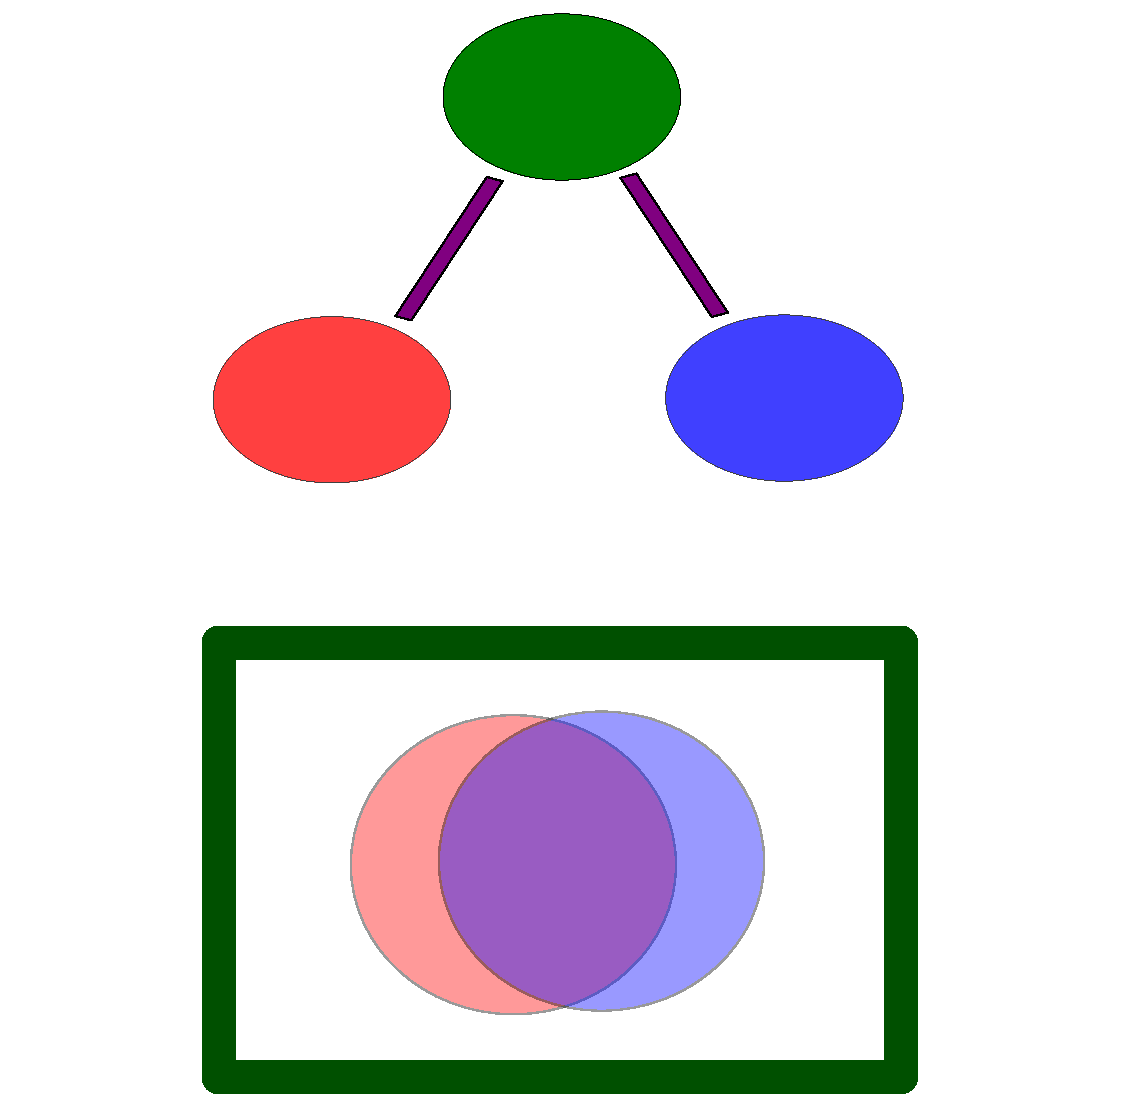
\includegraphics[width=0.3\textwidth]{teaims/Redundancy_Trimming_Ontology.pdf}
    }
  \subbottom{%
    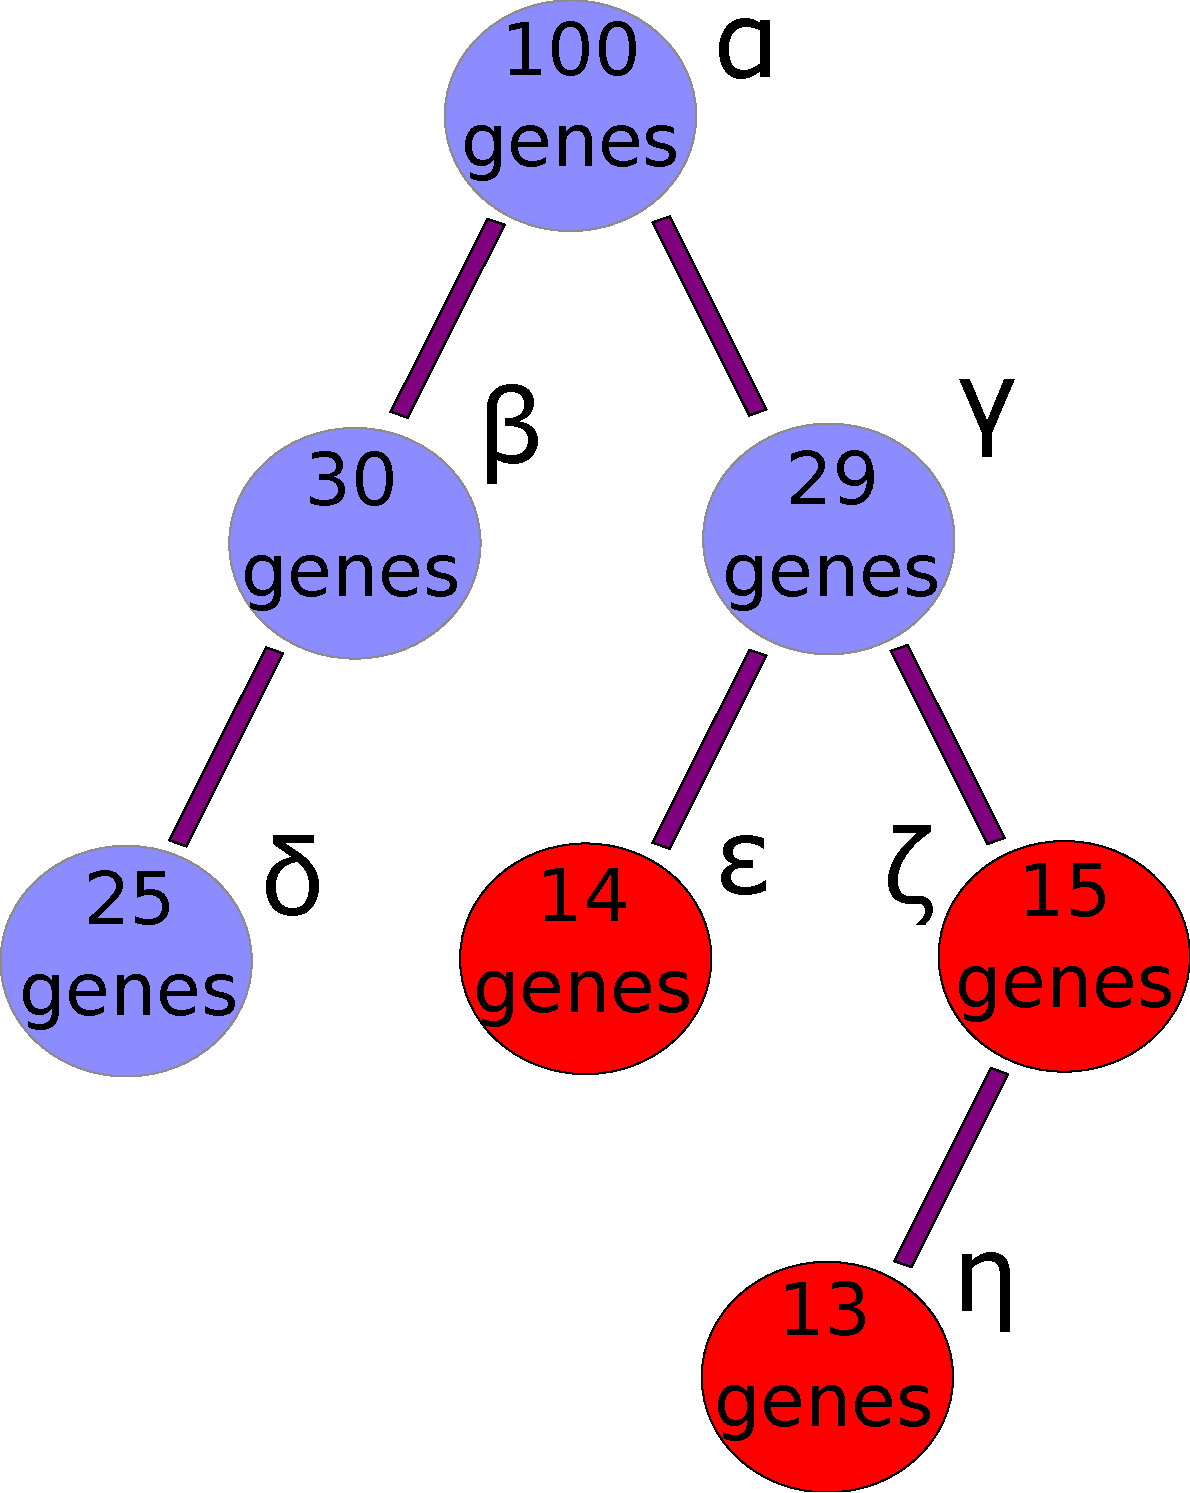
\includegraphics[width=0.3\textwidth]{teaims/Floor_Trimming_Ontogeny.pdf}
    }
  \subbottom{%
    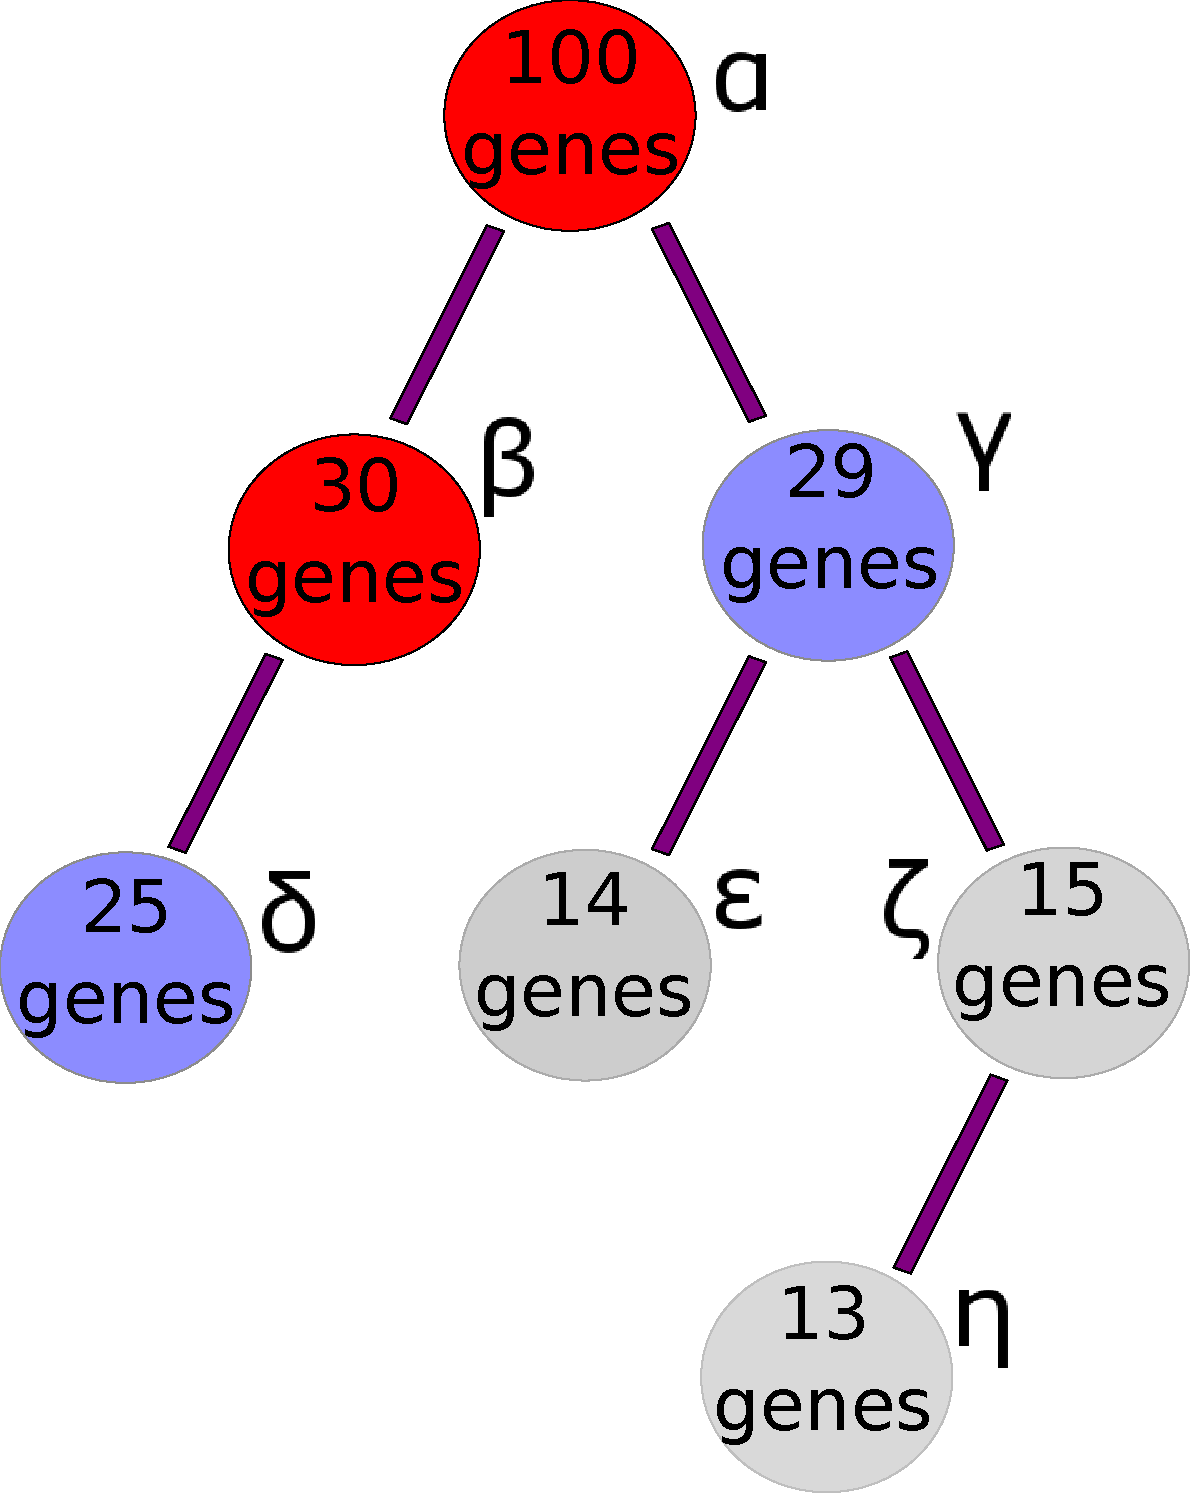
\includegraphics[width=0.3\linewidth]{teaims/Ceiling_Trimming_Ontology.pdf}
    }
  \caption{Schematic representation of trimming filters for an acyclical
           ontology.
    \textbf{a.}
    The parent node (green) contains at least as many
    annotations as the union of the two sisters. These two sisters share
    annotations extensively, as expressed by the overlap in the Venn diagram,
    so they qualify for removal.
  	\textbf{b.}
    Nodes with less than a threshold number of genes are
    trimmed (red) and discarded from the dictionary. Here, the example threshold
    is 25 genes. Nodes $\epsilon, \zeta, \eta$, shown in red are removed.
  	\textbf{c.}
    Parent nodes are removed recursively, starting from
    the root, if all their daughter nodes have more than the threshold number of
    annotations. Nodes in grey ($\epsilon, \zeta, \eta$) were removed in the
    previous step. Nodes $\alpha, \beta$ shown in red are trimmed because each one
    has a complete daughter set. Only nodes $\gamma$ and $\delta$ will be used to
    generate the static dictionary.}
\label{fig:simdiagram}
\end{figure}


\subsubsection*{Terminal branch terms and parent terms can be
safely removed in an algorithmic fashion }
Another problem arises from the ontology being scarcely populated. Many nodes
have 0--10 annotations, which we consider too few to accurately test. To solve
this issue, we implemented another straightforward node selection strategy. For
a given terminal node, we test whether the node has more than a threshold number
of annotations. If it does not, the node is not used for statistical testing.
The next higher node in the branch is tested and removed recursively until a
node that satisfies the condition is found. At that point, no more nodes can be
removed from that branch. This completion is guaranteed by the structure of the
ontology: parent nodes inherit all of the annotations of all of their
descendants, so the number of annotated terms monotonically increases with
increasing term hierarchy (see Figure~\ref{fig:simdiagram}). In this way, we
ensure that our term dictionary includes only those tissues that are considered
sufficiently well annotated for statistical purposes.

Additionally, we reasoned that for any parent node if all its daughters were
selected for testing, there was no additional benefit to test the parent. We
removed parent nodes from the analysis if all their daughter nodes passed the
annotation threshold (see Figure~\ref{fig:simdiagram}). We called this a ceiling
filter. Applying these three filters reduced the number of ontology terms by an
order of magnitude.

\subsubsection*{Filtering greatly reduces the number of nodes used for analysis}
By itself, each of these filters can reduce the number of nodes employed for
analysis, but applying the filters in different orders removes different numbers
of nodes (not all the filters are commutative). We chose to always execute
annotation and similarity thresholding first, followed by the ceiling filter.
%If the ceiling filter is applied before any other filter, only terminal nodes
% will remain, since all the parents have complete daughter sets. Since terminal
% nodes are the most poorly annotated, after applying the remaining filters very
% few nodes will be left behind if any. On the other hand, applying the ceiling
% operator after trimming and redundancy filtering will result in greater numbers
% f nodes. We always applied the ceiling at the end.
For validation (see below) we made a number of different dictionaries. The
original ontology has almost 6,000 terms of which 1675 have at least 5 gene
annotations. After filtering, dictionary sizes ranged from 21 to a maximum of
460 terms, which shows the number of terms in a scarcely annotated ontology can
be reduced by an order of magnitude through the application of a few simple
filters (see Table~\ref{tab:DictionarySpecs}). These filters were used to compile
a static dictionary that we employ for all analyses (see \emph{Validation of the
algorithm and parameter selection} section for details). Our trimming pipeline is
applied as part of each new WormBase release. This ensures that the ontology
database we are using remains up-to-date with regards to both addition or removal
of specific terms as well as with regard to gene expression annotations.

\begin{table}[p]
	\caption{
	Parameter specifications and number of tissues for all dictionaries. The
  `Method' column refers to the trimming criterion for the similarity metric.
  We used two such criteria, `any' and `avg'.`any': For a given sister set, if
  any sister had a similarity exceeding the corresponding threshold, all sisters
  were removed from the final dictionary. `avg': For a given sister set, if the
  average similarity across all the sisters in the set was greater than the
  corresponding threshold, all sisters were removed from the final dictionary.
	}
	\csvreader[tabular= c | c | c | c,
	table head= {\textbf{Annotation Cutoff}} & {\textbf{Similarity Threshold}}
  & {\textbf{Method}} & {\textbf{No. Of Terms in Dictionary}}\\\toprule,
	late after line= \\,
	late after last line= \\\hline
	]
	{tables/TissueNumbers.csv}{}
	{\csvcoli & \csvcolii & \csvcoliii & \csvcoliv}

\label{tab:DictionarySpecs}
\end{table}

\subsection*{Tissue enrichment testing via a hypergeometric model}
Having built a static dictionary, we generated a Python script that implements a
significance testing algorithm based on the hypergeometric model. Briefly, the
hypergeometric model tests the probability of observing $n_i$ occurences of a
tissue $i$ in a list of size $M$ if there are $m_i$ labels for that tissue in a
dictionary of total size $N$ that are drawn without replacement. Mathematically,
this is expressed as:

\begin{eqnarray}\label{hypergeometric}
	\mathrm{P}(n_i | N, m_i, M) = \frac{\dbinom{m_i}{n_i}
  \dbinom{M-m_i}{N - n_i}}{\dbinom{N}{n_i}}\text{.}
\end{eqnarray}

Although a user will input gene IDs, we test the number of ocurrences of a term
within the gene list, so a single gene can contribute to multiple terms. Due to
the discrete nature of the hypergeometric distribution, this algorithm can
generate artifacts when the list is small. To avoid spurious results, a tissue is
never considered significant if there are no annotations for it in the
user-provided list.

Once the p-values for each term have been calculated, we apply a standard FDR
correction using a Benjamini-Hochberg step-up algorithm~\citep{Benjamini1995}.
FDR corrected p-values are called q-values. Genes that have a q-value less than
a given alpha are considered significant. Our default setting is an alpha of 0.1,
which is a standard threshold broadly agreed upon by the scientific community
(see for example~\citep{Love2014, Pawitan2005, Storey2003}). This threshold cannot
be altered in the web GUI, but is user tunable through our command-line
implementation.

Users input a gene list using any valid gene name for \emph{C.~elegans}. These
names are processed into standard WormBase gene IDs (WBGene IDs). The program
returns a table containing all the enriched terms and associated  information
such as number of terms in gene list and expected number of terms. Finally, the
program can also return a bar chart of the enrichment fold change for the fifteen
tissues with the lowest measured q-values. The bars in the graph are sorted in
ascending order of q-value and then in descending order of fold-change. Bars are
colored for ease of viewing, and color does not convey information. Our software
is implemented in an easy to use GUI (see Figure~\ref{fig:GUIresults}). Anatomy
terms are displayed in human-readable format followed by their unique ontology
ID (WBbt ID). In summary, each time the ontology annotations are updated, a new
trimmed ontology is generated using our filters; in parallel, users can submit
their gene lists through WormBase for testing, with results output in a number
of formats (see Figure~\ref{fig:workflow}).

%gui
\begin{figure}[htbp]
	\centering
    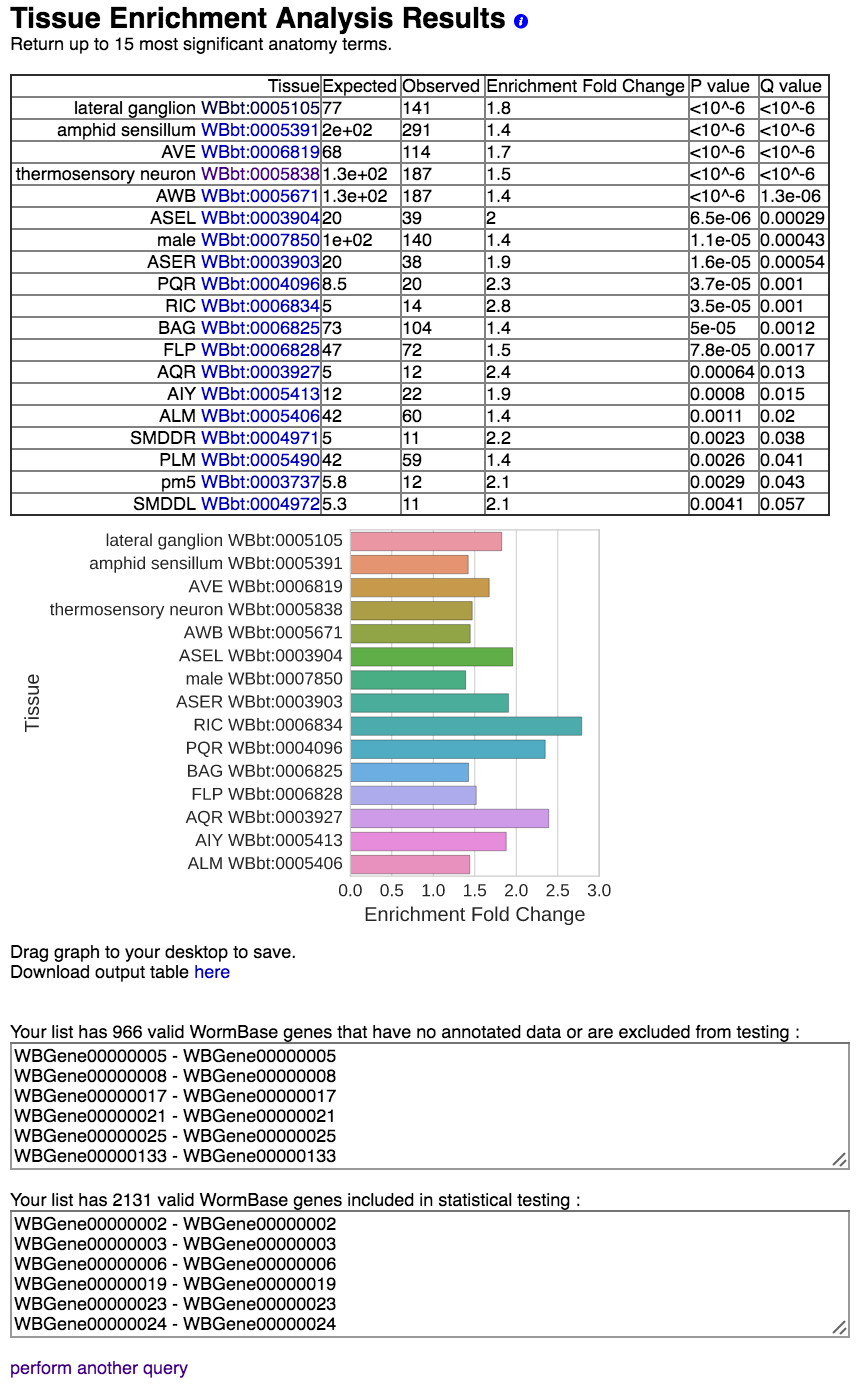
\includegraphics[width=0.5\textwidth]{teaims/guiresults.png}
 	\caption{
  Screenshot of results from the web GUI.
	After inputting a gene-list, the user is provided with the results. An HTML
  table is output with hyperlinks to the ontology terms. A publication-ready
  graph is provided below, which can be saved by  dragging to the desktop. The
  graph is colored for better visualization; color is not intended to convey
  information. The graph and the table show anatomy terms in  human-readable
  format, followed by their unique WBbt ID.\@ Finally, lists  of the genes used
  and discarded for the analysis are also presented.}
\label{fig:GUIresults}
\end{figure}

% workflow
\begin{figure}[htbp]
	\centering
	\includegraphics[width=0.95\textwidth]{teaims/workflow.pdf}
	\caption{
	TEA Workflow.
	The complete ontology is annotated continuously by WormBase curators. After
  each update, the ontology is processed to remove uninformative terms, and the
  remaining terms are used for statistical testing.
	Users can select a gene list and input it into our tool using our WormBase
  portal. The gene list is tested for enrichment using the trimmed ontology, and
  results are output in tabular and graphic formats for analysis.}
\label{fig:workflow}
\end{figure}



\subsection*{Validation of the algorithm and optimizing parameter selection}
We wanted to select a dictionary that included enough terms to be specific beyond
the most basic \emph{C.~elegans} tissues, yet would minimize the number of
spurious results and which had a good dynamic range in terms of enrichment
fold-change. Larger tissues are correlated with better annotation, so increasing
term specificity is associated with losses in statistical power. To help us
select an appropriate dictionary and validate our tool, we used a set of 30 gold
standards based on microarray and RNA-seq literature which are believed to be
enriched in specific tissues~\citep{Gaudet2004a, Spencer2011, Cinar2005,
Watson2008a, Pauli2006, Portman2004, Fox2007, Smith2010}. These data sets are
annotated gene lists derived from the corresponding Expression Cluster data in
WormBase. Some of these studies have been used to annotate gene expression, and
so they did not constitute an independent testing set. To correct this flaw, we
built a clean dictionary that specifically excluded all annotation evidence that
came from these studies.

As a first attempt to select a dictionary, we generated all possible combinations
of dictionaries with minimal annotations of 10, 25, 33, 50 and 100 genes and
similarity cutoffs of 0.9, 0.95 and 1, using `avg' or `any' similarity
thresholding methods (see Table~\ref{tab:DictionarySpecs}). The number of
remaining ontology terms was inversely correlated to the minimum annotation
cutoff, and was largely insensitive to the similarity threshold in the range we
explored. Next, we analyzed all 30 datasets using each dictionary. Because of
the large number of results, instead of analyzing each set of terms individually,
we measured the average q-value for significantly enriched terms in each dataset
without regard for the perceived accuracy of the terms that tested significant.
We found that the similarity threshold mattered relatively little for any
dictionary. We also noticed that the `any' thresholding method resulted in
tighter histograms with a mode closer to 0. For this reason, we chose the `any'
method for dictionary generation. The average q-value increased with decreasing
annotation cut-off (see Figure~\ref{fig:qvals}), which reflects the decreasing
statistical power associated with fewer annotations per term, but we remained
agnostic as to how significant is the trade-off between power and term
specificity. Based on these observations, we ruled out the dictionary with the
100 gene annotation cut-off: it had the fewest terms and its q-values were not
low enough in our opinion to compensate for the trade-off in specificity.

%q plot
\begin{figure}[htbp]
	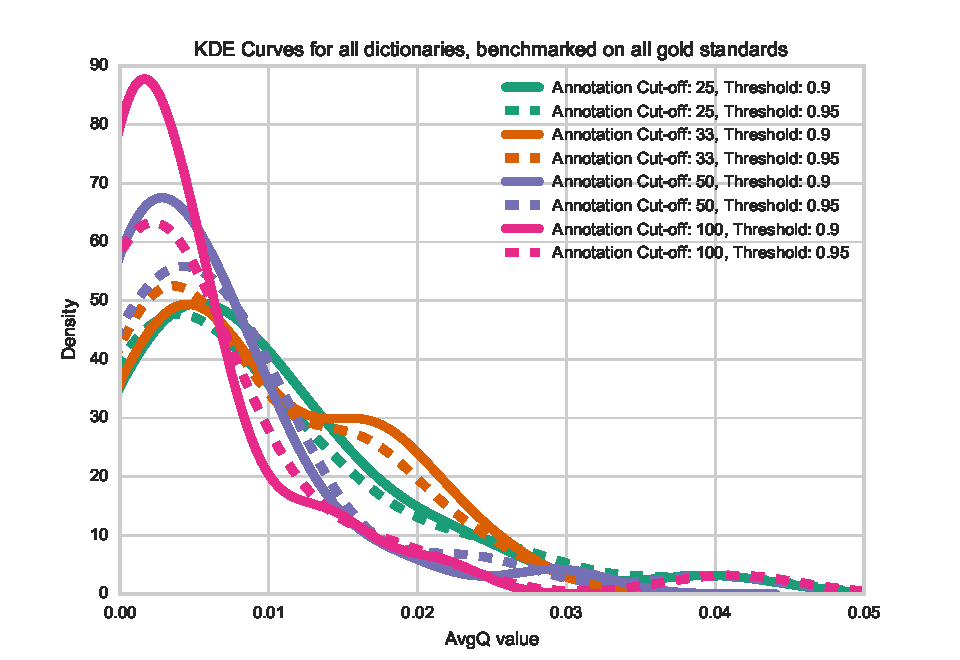
\includegraphics[width=.6\textwidth]{teaims/avgQKDE_method=any.pdf}
  \caption{
  Kernel density estimates (KDE) for 30 gold standard datasets.
  We ran TEA on 30 datasets we believed to be enriched in particular tissues
  and pooled all the results to observe the distribution of q-values. The
  mode of the distribution for dictionaries with annotation cut-offs of 100
  and 50 genes are very similar; however, when the cut-off is lowered to 25
  genes, the mode of the distribution shifts to the left, potentially
  signalling a decrease in measurement power.}
\label{fig:qvals}
\end{figure}


%dictionaries that work well
To select between dictionaries generated between 50, 33 and 25 annotation
cut-offs, and also to ensure the terms that are selected as enriched by our
algorithm are reasonable, we looked in detail at the enrichment analysis results.
Most results were comparable and expected. For some sets, all dictionaries
performed well. For example, in our `all neuron enriched sets'~\citep{Spencer2011,
Watson2008a} all terms were neuron-related regardless of the dictionary used
(see Table~\ref{tab:intraagree}). On the other hand, for a set enriched for
germline precursor expression in the embryo~\citep{Spencer2011}, the 50 cutoff
dictionary was only able to identify `oocyte WBbt:006797', which is not a
germline precursor although it is germline related; whereas the two smaller
dictionaries singled out actual germline precursor cells---at the 33 cutoff, our
tool identified the larval germline precursor cells `Z2' and `Z3' as enriched,
and at the 25 gene cutoff the embryonic germline precursor terms `P$_4$',`P$_3$'
and `P$_2$' were identified in addition to `Z2' and `Z3'.
%Differences between dictionaries
We also queried an intestine precursor set~\citep{Spencer2011}. Notably, this
gene set yielded no enrichment when using the 25 cutoff dictionary, nor when
using the 50 cutoff dictionary. However, the 33 cutoff dictionary identified the
E lineage, which is the intestinal precursor lineage in \emph{C.~elegans}, as
enriched. Both of these results capture specific aspects of \emph{C.~elegans}
that are well known to developmental biologists.

\begin{table}[p]
	\caption{
	Comparison of results for a GABAergic neuronal-enriched gene set from
  Watson~\citep{Watson2008a} showing that results are similar regardless of
  annotation cutoff. We ran the same gene list on a dictionary with a minimum
  annotation cutoff of 50, similarity threshold of 0.95 and similarity method
  `any' versus another with a minimum annotation cutoff of 33, similarity
  threshold of 0.95 and similarity method `any'. In the table, columns are
  abeled with their significance value (Q-value) or enrichment fold change
  followed by a hyphen and a number which indicates which the cutoff for the
  dictionary that was used for testing. Not all tissues are present in either
  dictionary. Hyphens denote not-applicable values, which occurs when a
  particular tissue is not present in both dictionaries.
	}
\label{tab:intraagree}
\end{table}

%Bad stuff.
Not all queries worked equally well. For example, a number of intestinal
sets~\citep{Spencer2011, Pauli2006} were not enriched in intestine-related terms
in any dictionary, but were enriched for pharynx and hypodermis. We were
surprised that intestinal gene sets performed poorly, since the intestine is a
relatively well-annotated tissue.

%Dictionary intra-agreement
We assessed the internal agreement of our tool by using independent gene sets
that we expected to be enriched in the same tissues. We used two  pan-neuronal
sets~\citep{Spencer2011, Watson2008a}; two PVD sets~\citep{Spencer2011, Smith2010};
and two  GABAergic sets~\citep{Spencer2011, Cinar2005}. Overall, the tool has
good internal agreement. On most sets, the same terms were enriched, although
order was somewhat variable (see Table~\ref{fig:interagree}), and most
high-scoring terms were preserved between sets. All comparisons can be found
online in our Github repository (see Availability of data and materials).
Overall, the dictionary generated by a 33 gene annotation cutoff with 0.95
redundancy threshold using the `any' criterion performed best, with a good
balance between specificity, verbosity and accuracy, so we selected this
parameter set to generate our static dictionary. As of this publication, the
testable dictionary contains 261 terms.

%gaba
\begin{figure}
	\centering{}
  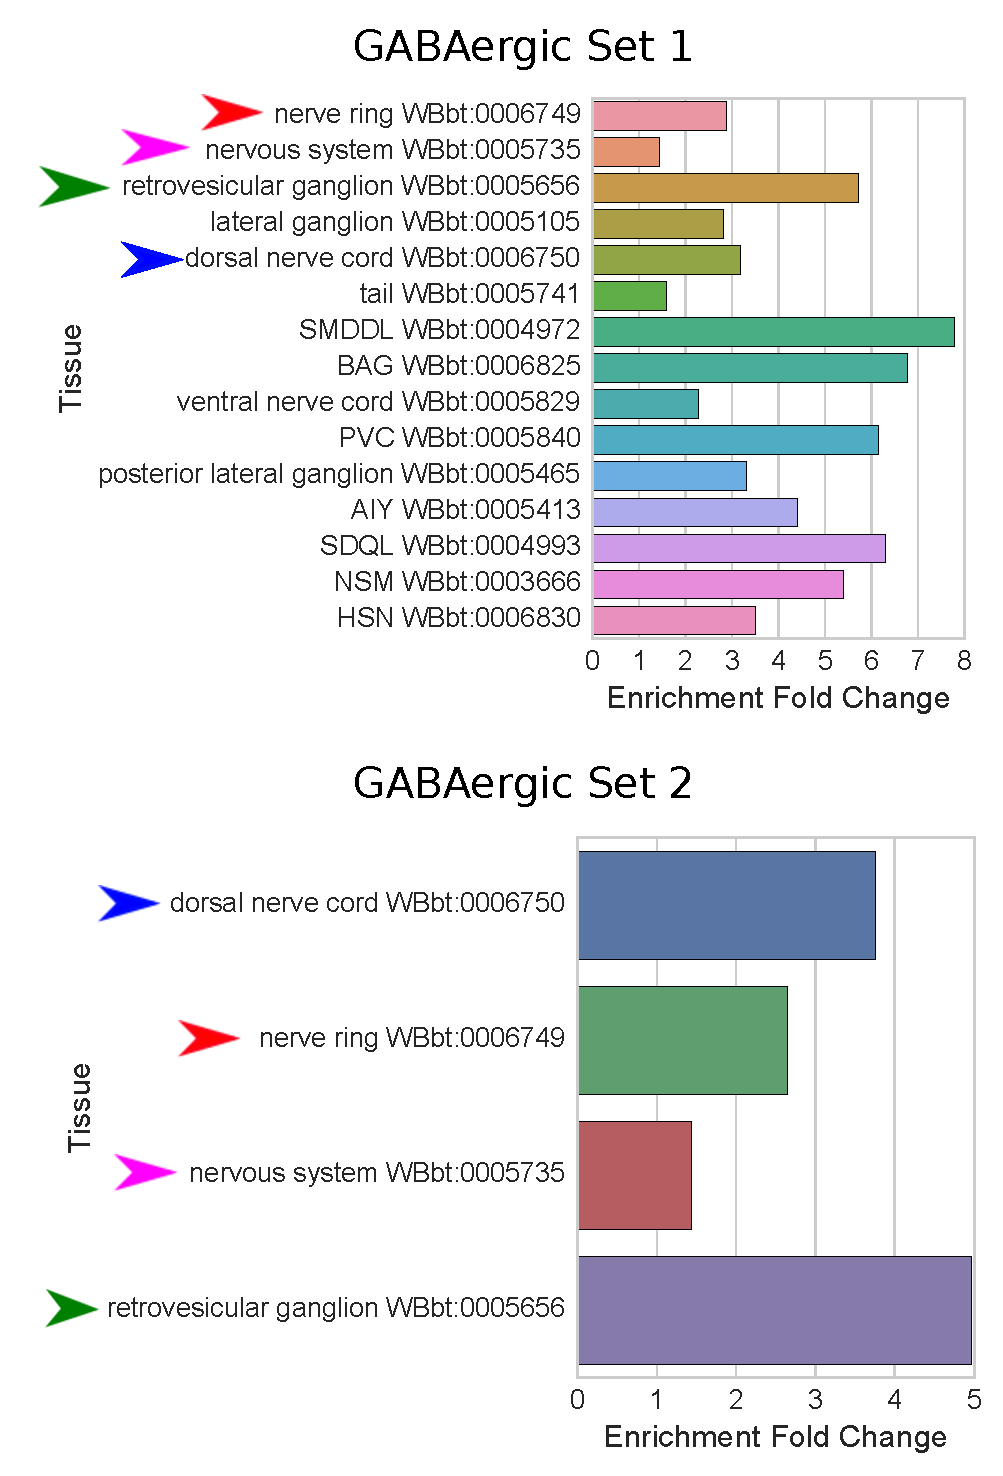
\includegraphics[width=0.6\textwidth]{teaims/GABAcomparison3.pdf}
  \caption{
  Independently derived gene sets show similar results 	when tested
  with the same dictionary.
  \textbf{Set 1.} GABAergic gene set from Watson~\citep{Watson2008a}.
  \textbf{Set 2.} GABAergic gene set from Spencer~\citep{Spencer2011}.
  Arrowheads highlight identical terms between both analyses. All terms refer to
  neurons or neuronal tissues and are GABA-associated. Dictionary with cutoff:
  33; threshold: 0.95; method: `any'.}
\label{fig:interagree}
\end{figure}


\subsection*{Applying the tool}
We applied our tool to the RNA-seq datasets developed by Engelmann et
al.~\citep{Engelmann2011} to gain further understanding of their underlying
biology. Engelmann et al.\_ exposed young adult worms to 5 different pathogenic
bacteria or fungi for 24 hours, after which mRNA was extracted from the worms
for sequencing. We ran TEA on the genes Engelmann \emph{et al} identified as
up- or down-regulated. Initially we noticed that genes that are down-regulated
tend to be twice as better annotated on average than genes that were up-regulated,
suggesting that our understanding of the worm immune system is scarce, in spite
of important advances made over the last decade. Up-regulated tissues, when
detected, almost always included the hypodermis and excretory duct. Three of the
five samples showed enrichment of neuronal tissues or neuronal precursor tissues
among the down-regulated genes. As an independent verification, we also
performed GO analysis using PANTHER on the down-regulated genes for
\emph{D.~coniospora}. These results also showed enrichment in terms associated
with neurons (see Figure~\ref{fig:Dcon}). A possible explanation for this
neuronal association might be that the infected worms are sick and the neurons
are beginning to shut down; an alternative hypothesis would be that the worm is
down-regulating specific neuronal pathways as a behavioral response against the
pathogen. Indeed, several studies~\citep{Meisel2014, Zhang2005} have provided
evidence that \emph{C.~elegans} uses chemosensory neurons to identify pathogens.
Our results highlight the involvement of various \emph{C.~elegans} neuronal
tissues in pathogen defense.

\begin{figure}[htbp]
		\centering{}
    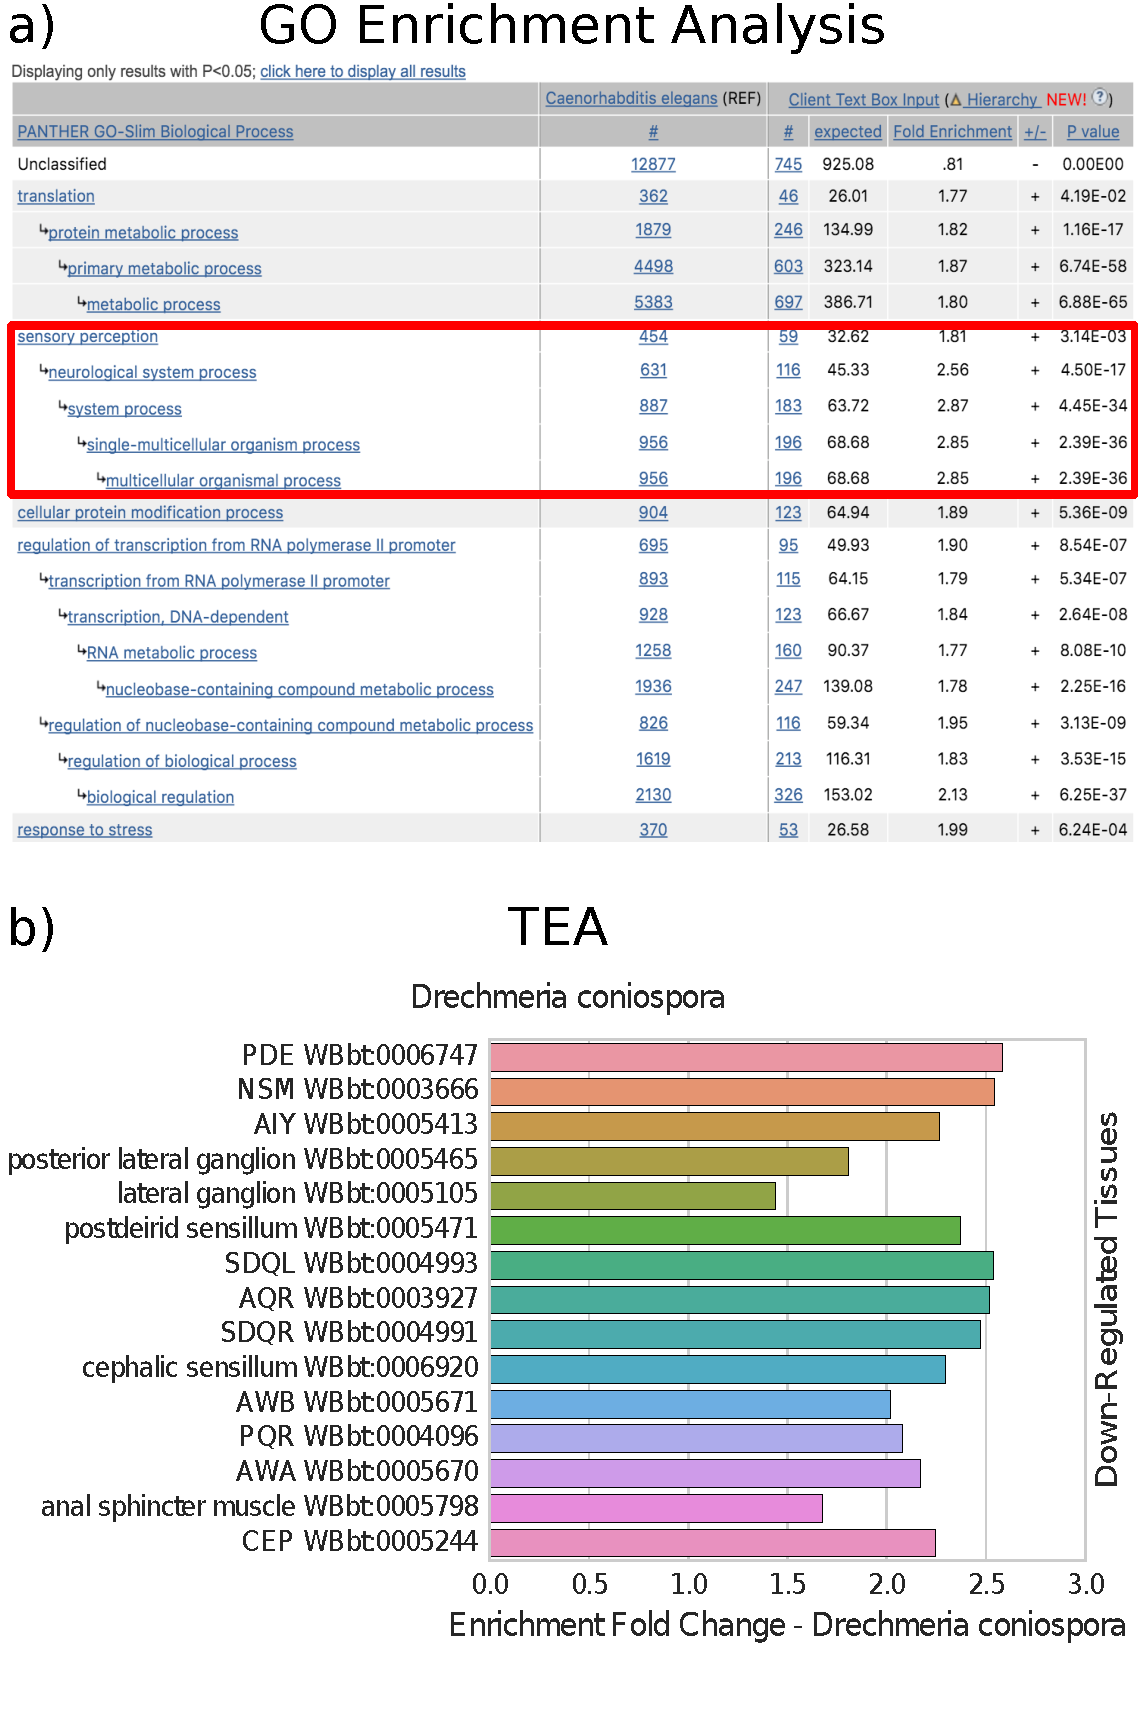
\includegraphics[width=0.65\textwidth]{teaims/engelmann-GO-tea-comparison.pdf}
  	\caption{
	\emph{D.~coniospora} Gene Enrichment Analysis and Tissue Enrichment
  Analysis results.
	We compared and contrasted the results from a gene enrichment analysis program,
  pantherDB, with TEA by analyzing genes that were significantly down-regulated
  when \emph{C.~elegans} was exposed to \emph{D.~coniospora} in a previously
  published dataset by Engelmann \emph{et al}~\citep{Engelmann2011} with both
  tools.
	\textbf{a.} pantherDB screenshot of results, sorted by p-value. Only top hits
  shown.
	\textbf{b.} TEA results, sorted by q-value (lowest on top) and fold-change.
	Both pantherDB and TEA identify terms associated with neurons (red square). The
  two analyses provide complementary, not redundant, information.
	}
\label{fig:Dcon}
\end{figure}


\section*{Discussion}
%TEA Discussion
We have presented a tissue enrichment analysis tool that employs a standard
hypergeometric model to test the \emph{C.~elegans} tissue ontology. We use a
hypergeometric function to test a user-provided gene list for enrichment of
anatomical terms in \emph{C.~elegans}. Our hope is that the physiological
relevance of anatomical terms will enable researchers to make hypotheses about
high-dimensionality data. Specifically, we believe an enriched term may broadly
suggest one of two hypotheses: if a list is enriched in a particular anatomical
region, that anatomical region is affected by the experimental treatment;
alternatively, the anatomical regions that are enriched reflect biologically
relevant interactions between tissues. We believe the first hypothesis is a
reasonable one to make in the case of whole-worm RNA-seq data for example,
whereas the second hypothesis may be more plausible in cases where a researcher
already knows what tissues a particular gene list came from, as may be the case
in single-cell RNA-seq.

%Other tools
Our tool relies on an annotation dictionary that is continuously updated
primarily with data from single gene qualitative analyses, does not require
retraining and does not require ranked genes. To our knowledge, this is the first
tool that tests tissue enrichment  in \emph{C.~elegans} via the hypergeometric
method, but similar projects exist for humans and zebrafish~\citep{Lee2013,
Prykhozhij2013}, highlighting the relevance of our tool for high-dimensionality
biology. Chikina \emph{et al}~\citep{Chikina2009} have previously reported a
tissue enrichment model for \emph{C.~elegans }based on a Support Vector Machine
classifier that has been trained on microarray studies. SVMs are powerful tools,
but they require continuous retraining as more tissue expression data becomes
available. Moreover, classifiers require that data be rank-ordered by some metric,
something which is not possible for certain studies. Furthermore, this tissue
enrichment tool provides users with enrichment results for only 6 large tissues.
In contrast, our tool routinely tests a much larger number of terms, and we have
shown it can even accurately identify enrichment of embryonic precursor lineages
for select data sets.

%Trimming discussion
We have also presented the first, to our knowledge, ontology term filtering
algorithm applied to biomedical ontologies. This algorithm, which is very easy
to execute, identifies terms that have specificity and statistical power for
hypothesis testing. Due to the nature of all ontologies as hierarchical, acyclical
graphs with term inheritance, term annotations are correlated along any given
branch. This correlation reduces the benefits of including all terms for
statistical analysis: for any given term along a branch, if that term passes
significance, there is a high probability that many other terms along that branch
will also pass significance. If the branch is enriched by random chance, error
propagation along a branch means that many more false positives will follow.
Thus, a researcher might be misled by the number of terms of correlated function
and assign importance to this finding; the fact that the branching structure of
GO amplifies false positive signals is a powerful argument for either reducing
branch length or branch intracorrelation, or both. On the other hand, if a term
is actually enriched, we argue that there is little benefit to presenting the
user with additional terms along that branch. Instead, a user will benefit most
from testing sparsely along the tree at a suitable specificity for hypothesis
formation. Related terms of the same level should only be tested when there is
sufficient annotation to differentiate, with statistical confidence, whether one
term is enriched above the other. Our algorithm reduces branch length by
identifying and removing nodes that are insufficiently annotated and parents
that are likely to include sparse information.


We endeavoured to benchmark our tool well, but our analysis cannot address
problems related to spurious term enrichment. Although we were unable to
determine false-positive and false-negative rates, we do not believe this should
deter scientists from using our tool. Rather, we encourage researchers to use our
tool as a guide, integrating evidence from multiple sources to inform the most
likely hypotheses. As with any other tool based on statistical sampling, our
analysis is most vulnerable to bias in the data set. For example, expression
reports are negatively biased against germline expression because of the
difficulties associated with expressing transgenes in this
tissue~\citep{Kelly1997}. As time passes, we are certain the accuracy and power
of this tool will improve thanks to the continuing efforts of the  worm research
community; indeed, without the community reports of tissue expression in the
first place, this tool would not be possible.

\section*{Conclusions}

We have built a tissue enrichment tool that employs a tissue ontology previously
developed by WormBase. We use a simple algorithm to identify the best ontology
terms for statistical testing and in this way minimize multiple testing problems.
Our tool is available within WormBase or can be downloaded for offline use via
`pip install'.

\section*{Methods}
\subsection*{Fetching annotation terms}
We used WormBase-curated gene expression data, which includes annotated
descriptions of spatial-temporal expression patterns of genes, to build our
dictionary. Gene lists per anatomy term were extracted from a Solr document
store of gene expression data from the WS252 database provided by
WormBase~\citep{Howe2016}. We used the Solr document store because it provided a
convenient access to expression data that included inferred annotations. That
is, for each anatomy term, the expression gene list includes genes that were
directly annotated to the term, as well as those that were annotated to the
term's descendant terms (if there were any). Descendant terms were those
connected with the focus term by is\_a/part\_of relationship chains defined in
the anatomy term ontology hierarchy.

\subsection*{Filtering nodes}
\subsubsection*{Defining a Similarity Metric}
To identify redundant sisters, we defined the following similarity metric:

\begin{eqnarray}
  \label{similarity def}
	s_i = \frac{|g_i|}{|\bigcup_{i= 0}^k g_i|}
\end{eqnarray}

Where $s_i$ is the similarity for a tissue $i$ with $k$ sisters; $g_i$ refers to
the set of tissues associated with tissue $i$ and $|g|$ refers to the
cardinality of set $g$. For a given set of sisters, we called them redundant if
they exceeded a given similarity threshold. We envisioned two possible criteria
and built different dictionaries using each one. Under a threshold criteron
`any' with parameter $S$ between $(0, 1)$, a given set of sisters $j$ was
considered redundant if the condition

\begin{eqnarray}
  \label{anythreshold}
	s_{i, j} > S
\end{eqnarray}

was true for any sister $i$ in set $j$. Under a threshold criterion `avg' with
parameter $S$, a given set of sisters $j$ was considered redundant if the
condition

\begin{eqnarray}
  \label{avgthreshold}
	\mathrm{E}[s_i]_{j} > S
\end{eqnarray}

was true for the set of sisters $j$ (see Figure~\ref{fig:simdiagram}).

Since nodes can have multiple parents (and therefore multiple sister sets), a
complete set of similarity scores was calculated before trimming the ontology,
and nodes were removed from the ontology if they exceeded the similarity
threshold at least once in any comparison.

\subsubsection*{Implementation}
All scripts were written in Python 3.5. Our software relies on the pandas, NumPy,
Seaborn and SciPy modules to perform all statistical testing and data
handling~\citep{McKinney2011, VanDerWalt2011, Oliphant2007}.


\section*{Availability of data and materials}
Our web implementation is available at
\url{http://www.wormbase.org/tools/enrichment/tea/tea.cgi}. Our software can also
be downloaded using Python's pip installer via the command

\texttt{pip install tissue\_enrichment\_analysis}

Alternatively, our software is available for download at:
\url{http://dangeles.github.io/TissueEnrichmentAnalysis}

All benchmark gene sets, benchmarking code and Figures can also be found at the
same address, under the `tests' folder.

\section*{Abbreviations}

\begin{itemize}
	\item TEA---Tissue Enrichment Analysis
	\item GO---Gene Ontology
	\item WBbt ID---A unique ID assigned to reference ontology terms
	\item WBgene ID---A unique ID assigned to reference nematode genes
\end{itemize}


% \section*{Ethics Approval and Consent to Participate}
% Not applicable
%
% \section*{Consent for Publication}
% Not applicable
%
% \section*{Competing interests}
%  	The authors declare that they have no competing interests.
% \section*{Author's contributions}
%     DA and PWS conceived of the project; DA developed algorithm;
% 	RYL made intellectual contributions to the project; RYL and JC
% 	developed the web GUI.
% \section*{Acknowledgements}
% 	We thank Justin Bois for his help and support.
% 	We would like to acknowledge all members of the Sternberg
% 	lab for helpful discussion.
% \section*{Funding}
% 	This work was supported by HG002223 from the National Human Genome Research
%   Institute to PWS., and H.H.M.I., with which PWS is an investigator. The
%   funding agencies had no input into the design, execution or interpretation
%   of our experiments, nor into the writing of this manuscript.

%%%%%%%%%%%%%%%%%%%%%%%%%%%%%%%%%%%
\section*{Additional Files}
  \subsection*{Additional file 1 --- TEA Tutorial}
    Tutorial for users interested in using our software within a python script
  \subsection*{Additional file 2 --- Folder Structure for SI files 3 and 4}
    A file detailing the folder structure of the zipped folders 3 and 4.
  \subsection*{Additional file 3 --- Golden Gene Sets}
    A list of all the genes used for our benchmarking process.
  \subsection*{Additional file 4 --- Results}
    A folder containing a complete version of the results we generated for this
    paper.
